\subsection{Analysis of Quiz Results}

    %What the data said

    % Christine och Patrick berättade senare att i regel presterar Young Mentor lite bättre än CBT, enligt deras rakningar. (från iteratoin 1 - stämde detta?)

    % Relevans av att testa financial literacy: "Precis som med förra gruppen, verkar ekonomin vara det svåraste att förstå (dolda utgifter, hur gå med vinst), som youth." (från iteration 1)

% Important to be objective
% En diskussion om hur resultaten kan användas i praktiken är också i de flesta fall belysande och relevant i rapporter

% https://liu.se/ias/kontakta-oss?l=en

For the first time, automatic data collection was used, which increased the amount of quantitative data that could be analysed substantially. Below, the findings from each data analysis method are presented. There was one test group and one reference group, the difference being if they were allowed to consult the manuals or only use the feedback from the app.

\subsubsection{Quiz Results and Pre-Test Data Analysed in Google Sheets}
For results gathered and analysed within the Google Sheet, see figure \ref{fig:analysFarg3}. For a zoomed in version, see Appendix \ref{cha:appendix4}. Early observations from the pre-test data when inserted into Google Sheets was that a surprising number of cells were left blank. One user had not done the pre-test (see column for coach 220), where some had left questions unanswered (most commonly "Do you own a company?" (should have used the word "business"), plus "Hours of preperation" and "Occations for a youth session" (there is a tendency this might be because they were not proud of their answers, because of correlations with low quiz results).

\begin{figure}[h]
    \centering
    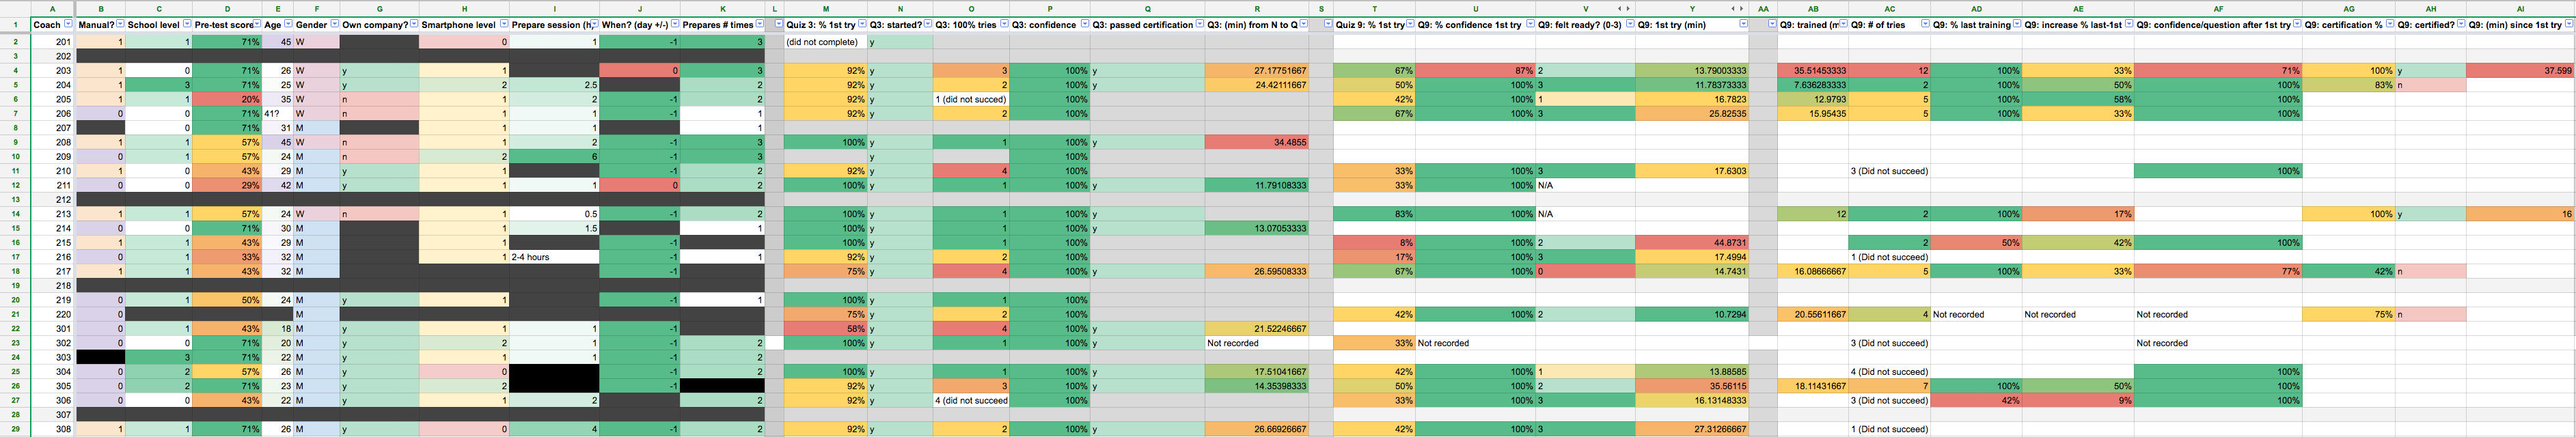
\includegraphics[width=1.0\textwidth]{analysis/sheets/0Overview.png}
    \caption{The Google Sheet after merging the pre-test data and the summed quiz results data. See zoomed-in versions and explanations for each section below.}
    \label{fig:analysFarg3}
\end{figure}

\begin{figure}[h]
    \centering
    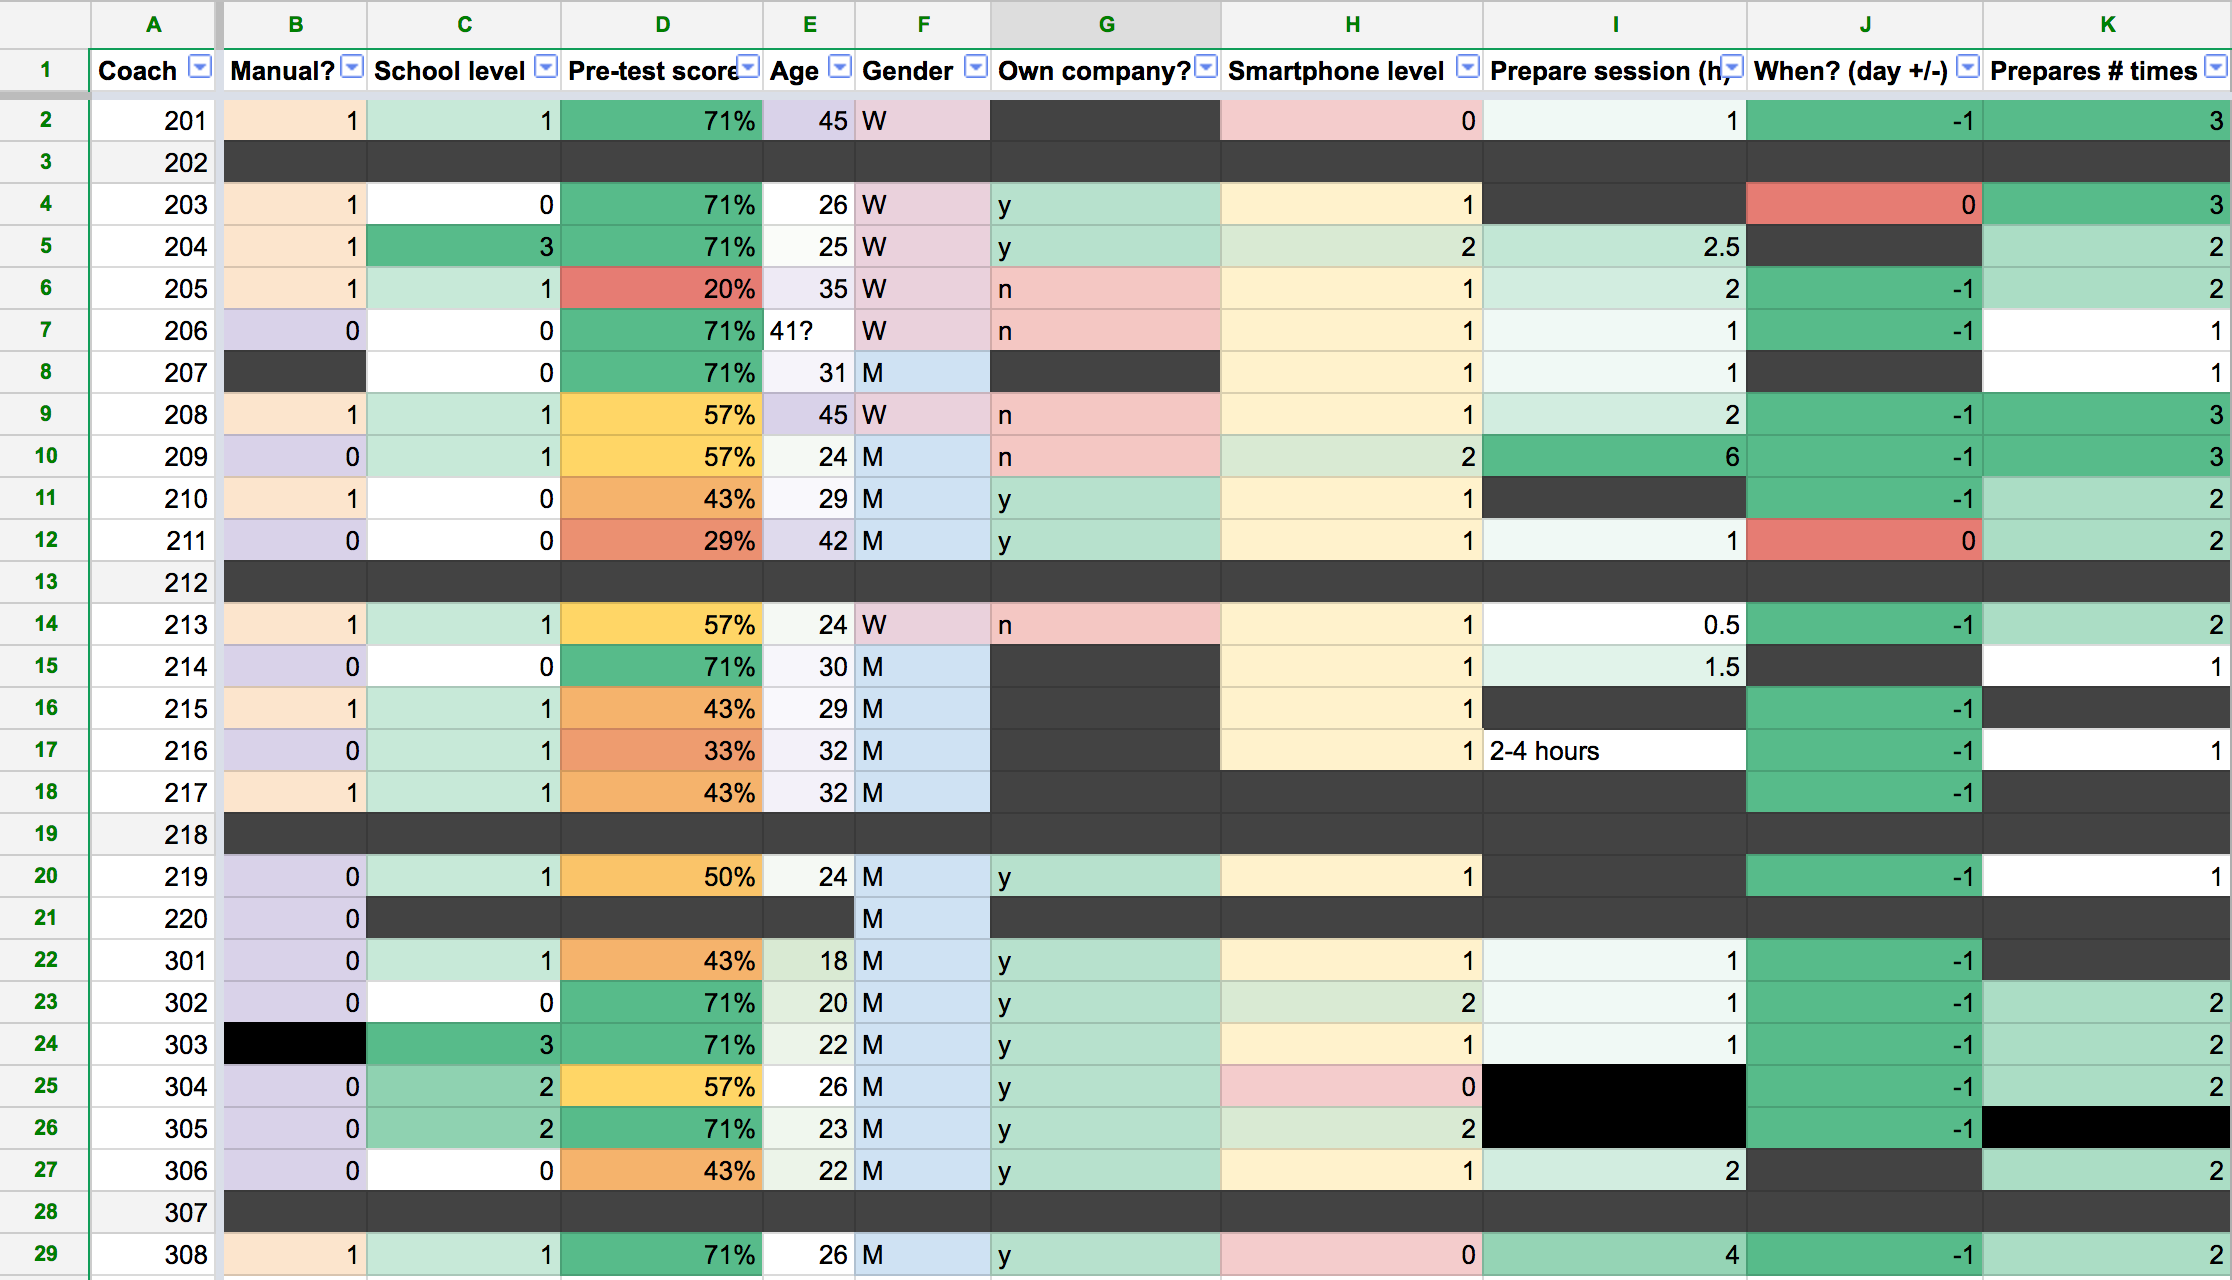
\includegraphics[width=1.0\textwidth]{analysis/sheets/1Pre-data.png}
    \caption{Pre-test data}
    \label{fig:1Pre-data}
\end{figure}

\begin{figure}[h]
    \centering
    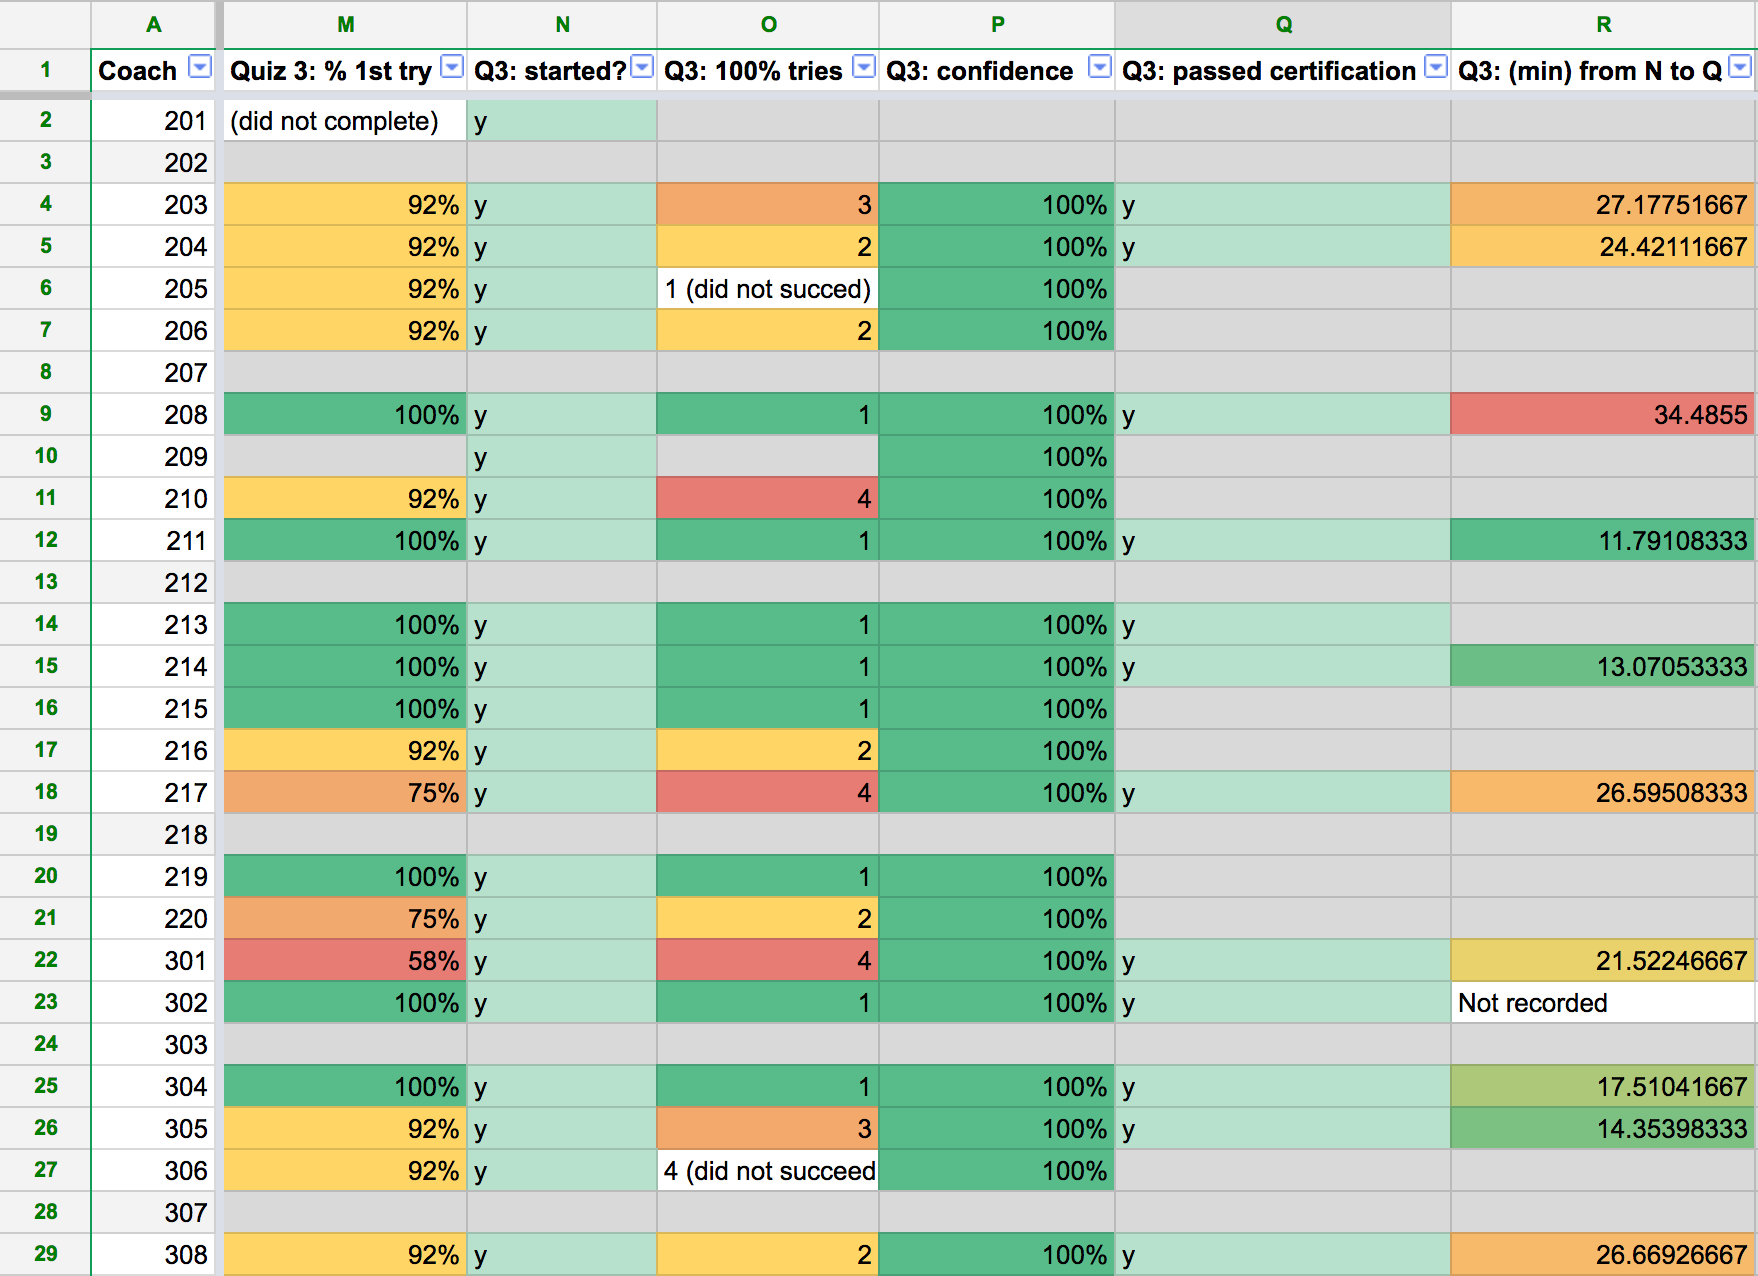
\includegraphics[width=1.0\textwidth]{analysis/sheets/2Quiz3.png}
    \caption{Quiz 3 answers.}
    \label{fig:2Quiz3}
\end{figure}

\begin{figure}[h]
    \centering
    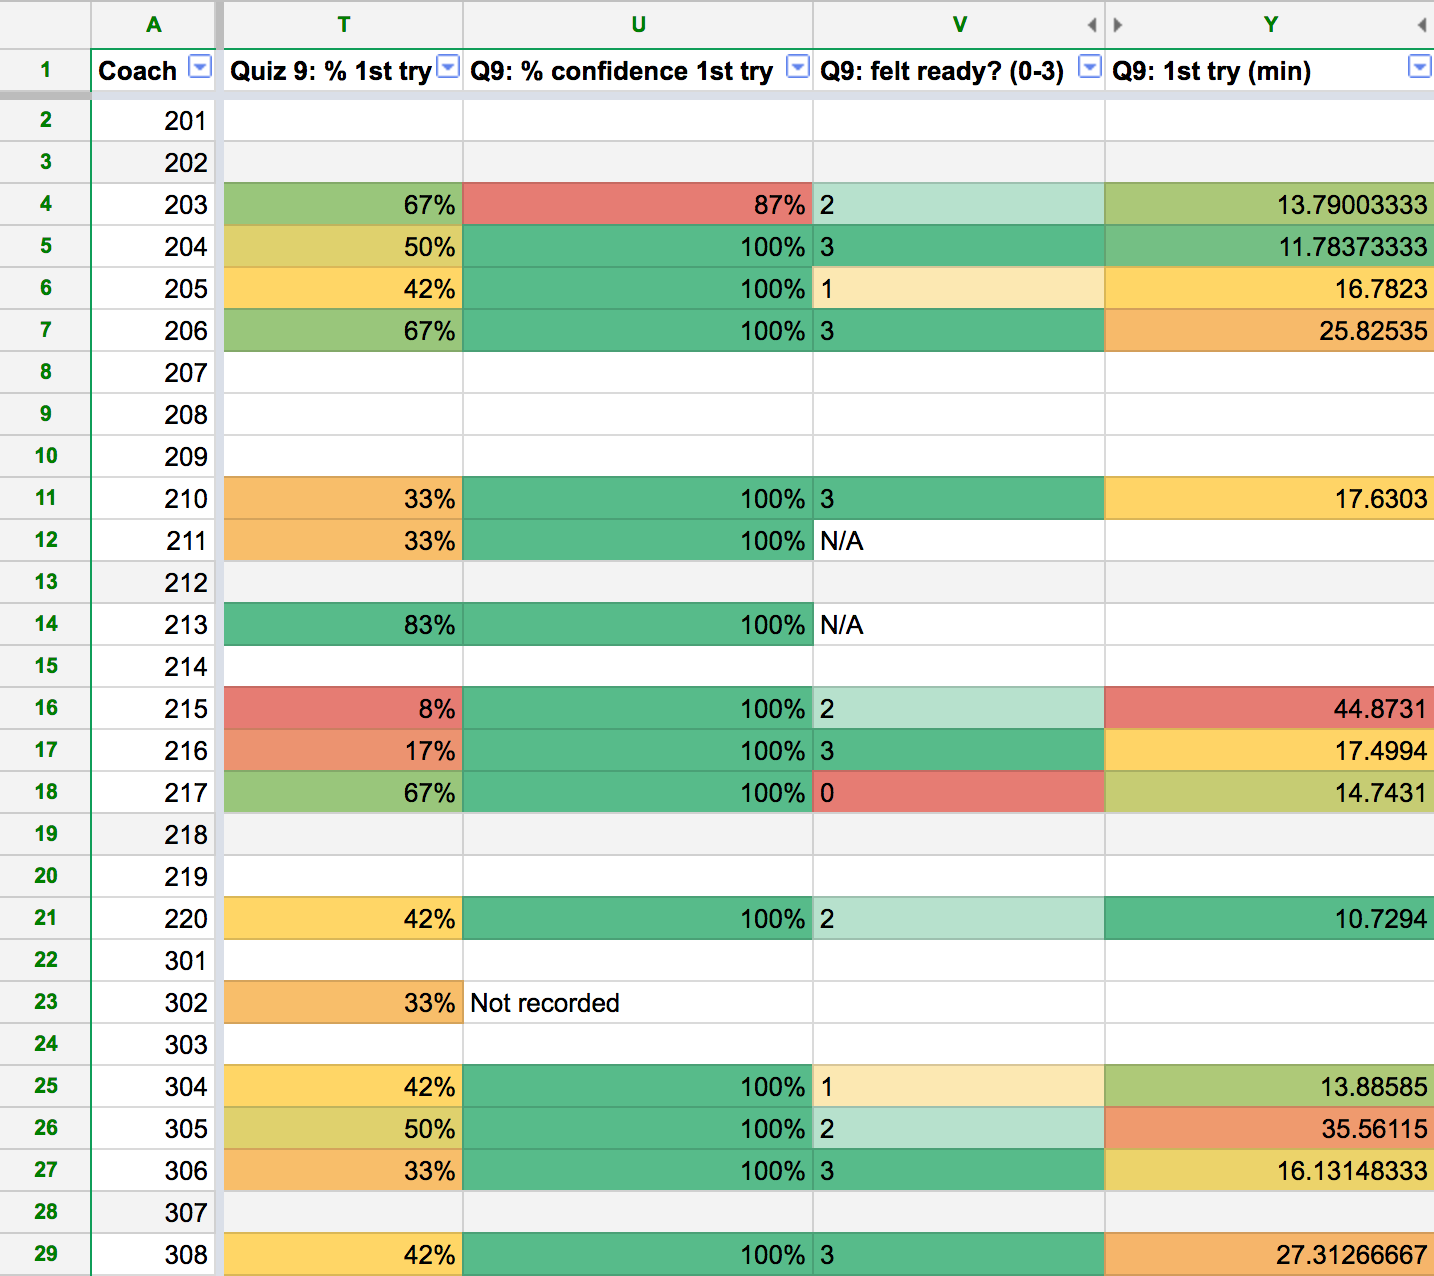
\includegraphics[width=1.0\textwidth]{analysis/sheets/3Quiz9A.png}
    \caption{Quiz 9 try 1 answers (correctness and recorded confidence ("Are you sure?": "Yes/No") on coach guide quiz 9 "Are you ready?", together with answering "How comfortable and ready do you feel right now to carry out session 9? (There is no right answer, just be honest with yourself!", alternative 1-4 ("Not ready at all", "Somehow ready", "Ready" or "Very ready and comfortable"). Finally in column Y, the time it took for the coach to complete quiz try 1 is given.}
    \label{fig:3Quiz9A}
\end{figure}

\begin{figure}[h]
    \centering
    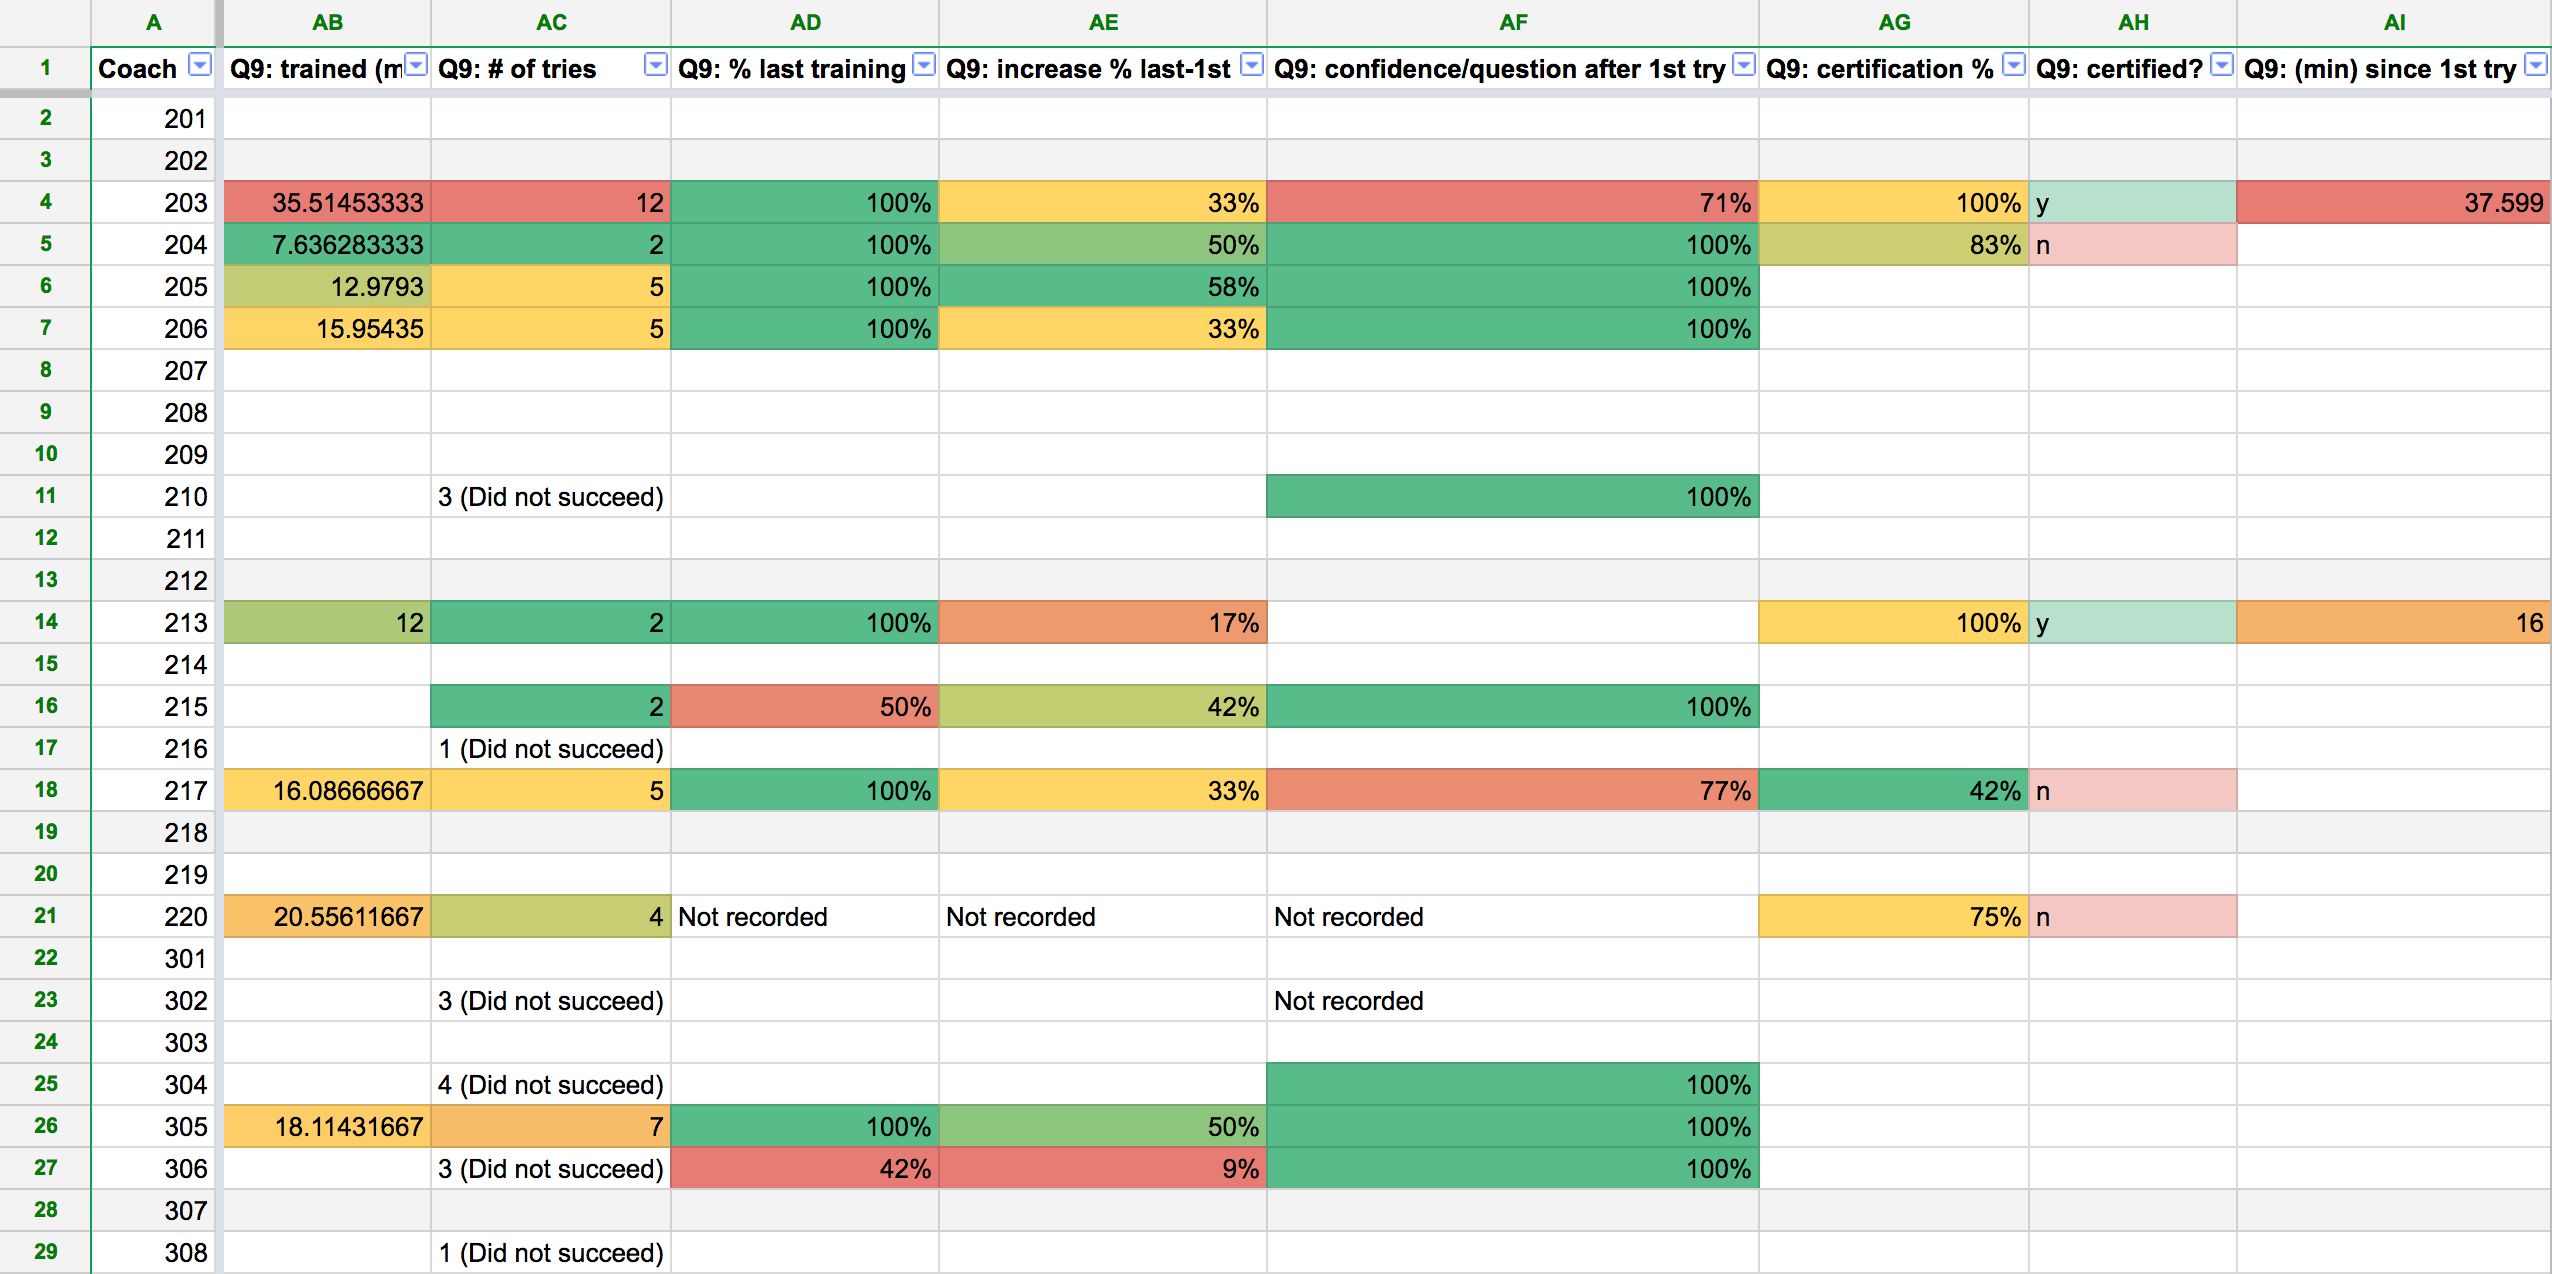
\includegraphics[width=1.0\textwidth]{analysis/sheets/3Quiz9B.png}
    \caption{Quiz results on the training and certification of coach guide quiz 9 "Are you ready?". Column AB: how many minutes they spent in training. AC: how many times they pressed "Try again", retaking the wrong answers. AD: their score on the last training quiz they took. AE: the increase from their first training to their last. AF: recorded "Are you sure?": "Yes/No" after taking the quiz try 1. Finally, for the coaches that started the certification, their results are shown, together with the time the quiz took for those that got 100\% correct on the first try.}
    \label{fig:3Quiz9B}
\end{figure}

\begin{figure}[h]
    \centering
    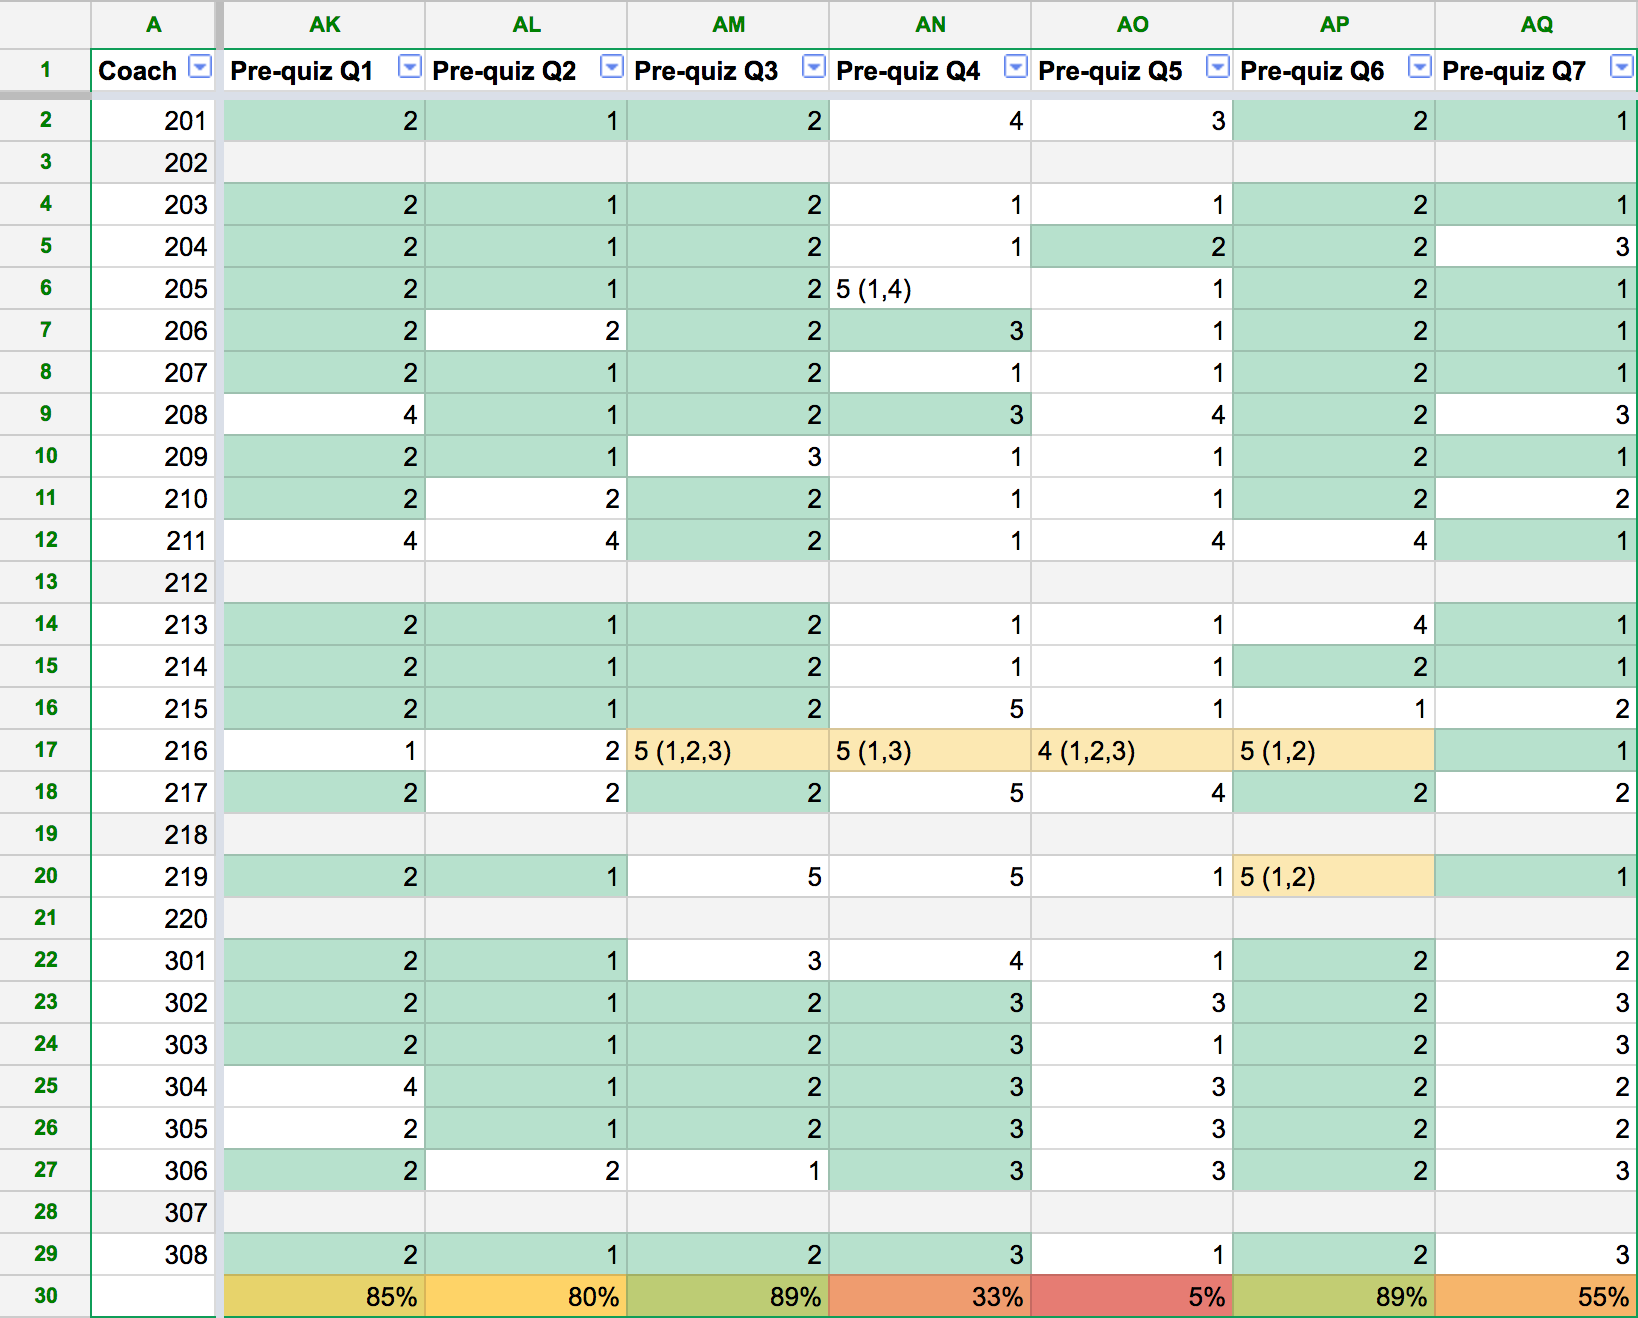
\includegraphics[width=1.0\textwidth]{analysis/sheets/4Pretest.png}
    \caption{Pre-quiz results per question and coach. The correct answers are given in green. The questions asked can be observed in Appendix \ref{cha:pre-test}}.
    \label{fig:4Pretest}
\end{figure}

\clearpage

Missing cells was not as obvious with the app results, were users could not progress in a quiz without answering both the question and the confidence. However, none of the passed quiz 9 certification answers had been submitted. Thus, it was needed to add these from the manual recordings, which had been used as a backup in case anything like this would happen.

There were a number of quick insights that could be drawn before the parallel coordinates visualization, simply by looking at the data as a spreadsheet.

It was believed that smartphone users feeling like novices might have a disadvantage with the app, since they will not learn as fast as experienced users. The interactions shows however, between iteration 3 to 4, almost all of the coaches does not feel intermediate instead of beginners using the smartphone and the YoungDrive app. The quiz data verifies this, with no direct correlation between technical skills and quiz results (comparing column H "Smartphone level" 1-3) with column M and T (quiz scores on the first try for quiz 3 and 9). From the pre-test data, it can be seen that only CBTs said they didn't feel comfortable with smartphone (n=2, column H, of which there were 6 Youth Mentors and 14 CBTs). A reason might be age, as CBTs were older than the Youth Mentors. Also, youth mentors had higher school level than the CBTs. More probable, is that the experience of using a smartphone since iteration 3 has matured over time, and that they are now more confident. %It is interesting that this has improved since iteration 3, possibly indicating that the smartphone skills have matured since the last test two weeks ago.

From the Google Sheets quiz results data, it could be seen that there was a surprisingly low number of answers where the user answered the question without confidence (see column P, U and AF). This is not good for feedback purposes, as answers were actually often not correct.

First-hand insights before the parallel coordinates were that there was a strong correlation between pre-quiz results (column D) and quiz 9 try 1 (column T), and slightly visible also in quiz 3 try 1 (column M), but with more outliers. Also, with manuals there was a higher probability of finishing quiz 9 training and certification (see also findings from the parallel coordinates visualization below). The data shows small tendencies that being honest and deliberate during the training increases the likelihood that a coach can get 100\% without faults, and has truly learned.

The final version of the app shows users can get 100\% on quiz results much faster (column R, AB and AI) than the previous version, as the score board had been improved for iteration 4. Since the target group in Zambia and Uganda was different, it is hard to empirically prove if it went faster getting 100\% with the possibility of repeating only the wrong questions, asking "Are you sure?", and providing individual feedback. Asking after the app does in iteration 4 does show however, that 100\% of the coaches now thought the feedback was good for learning.

%\subsubsection{Bonus Result: Learnings from Observing All of the Quiz Results}
Also, from observing all of the quiz submissions (see sample in figure \ref{fig:unprocessedData}), more users had started a quiz without finishing it than anticipated. This speaks for usability issues (cancelling the quiz by mistake, like clicking the back button, or loss of internet access) or bad technical skills (needs to design to be more fail-safe) or lack of motivation (needs to design for unmotivated coaches as well. The need group of "challenged coaches" might need other design than "ideal coaches".

Finally, a lot of users had done quizzes that were not Topic quiz 3 and Coach quiz 9, which might indicate high interest (if they did more than 2 quizzes) or confusion (if they did not do 3 or 9, but they did do other quizzes) during the app evaluation. This meant that on some aspects, there were less data than anticipated, (which was troublesome, as there were already few data points), and some aspects where there was more data than anticipated (on overlooked other quizzes).

\subsubsection{Parallel Coordinates Visualization}
Statistical analysis in R showed that none of the results were statistically significant to be notable using linear regression, or any of the other statistical methods detailed in the methodical framework. It was believed that statistical analysis could at least give insight into what to look for in the parallel coordinates visualization, but also for this, a larger sample would be needed. An interactive parallel coordinates visualization could give many more insights, more faster than the static presentations in Google Sheets or statistical analysis in R.

There is an almost infinite number of findings and observations that are interesting to look at via the parallel coordinates visualization. Even if there are no clear correlations (which are often found immediately when working with large data sets and parallel coordinates), tendencies can be found. As nothing is statistically significant (mostly because of the small data sample), the only thing that could be found are tendencies, and to analyze outliers. Then, these findings was critically analyzed to characteristics, and observations made from the app tests. As such, the data should be seen as indications of where future research is interested, and not as universal truths. For further research into the data, see figure \ref{fig:parallellCoordinates3} and the below sections.

\begin{figure}[h]
    \centering
    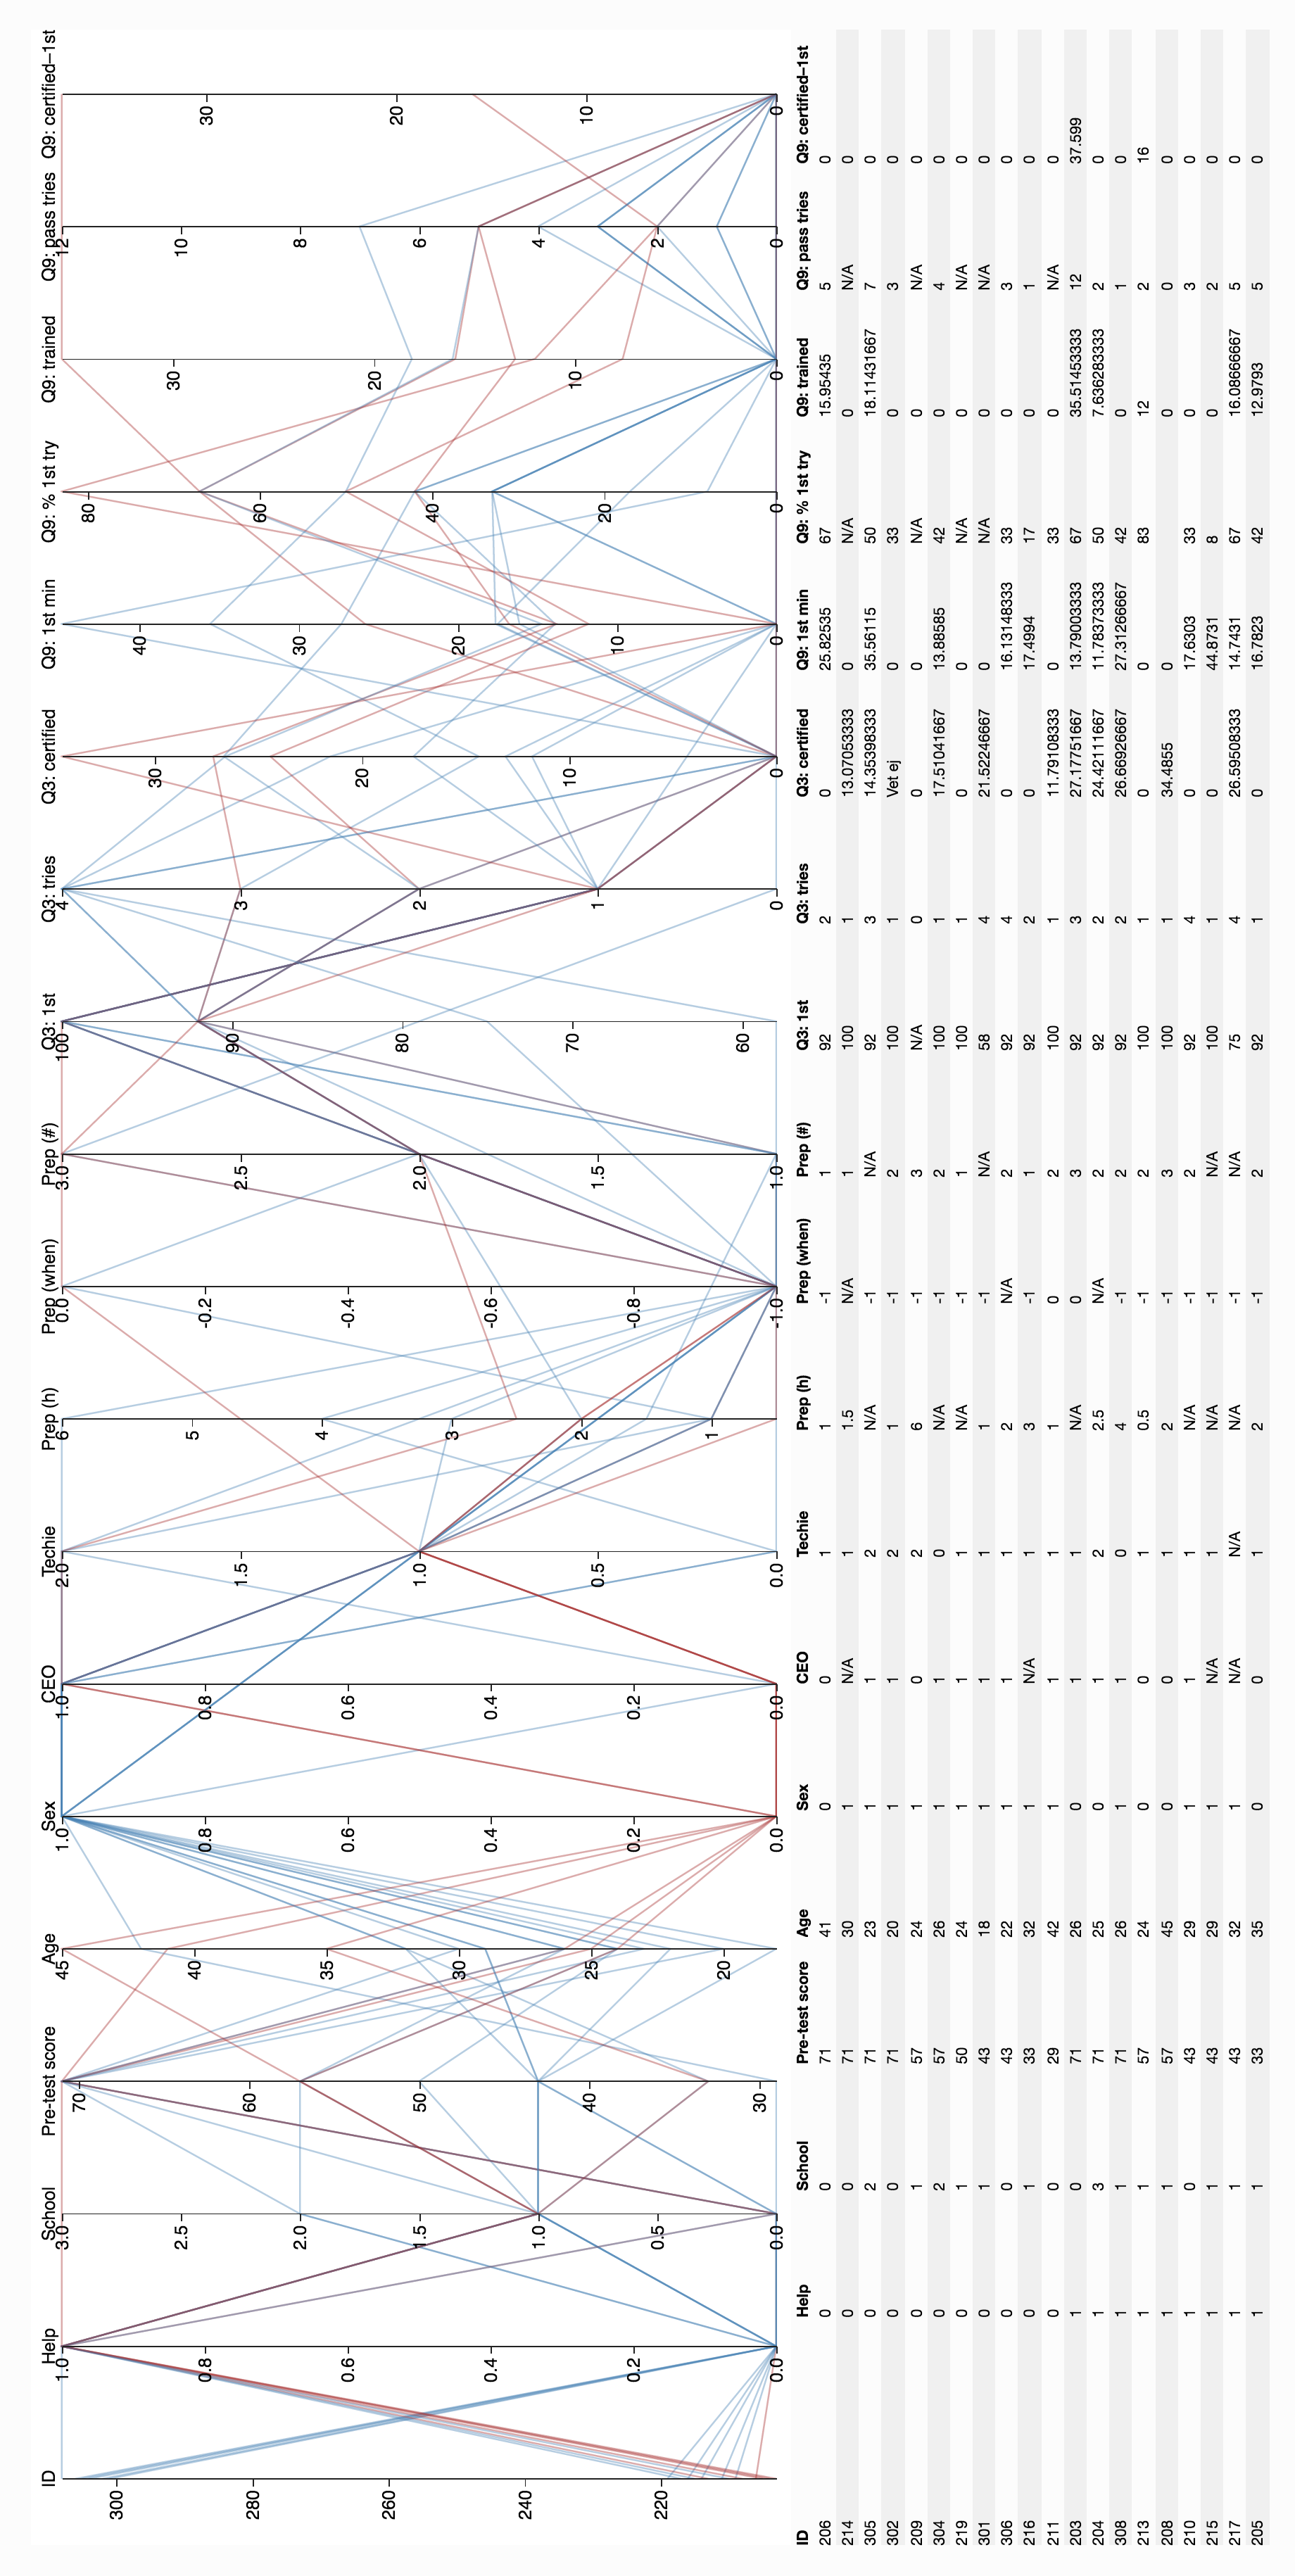
\includegraphics[width=0.7\textwidth]{analysis/parallellCoordinates3.png}
    \caption{The quiz results from iteration 4 shown in an interactive parallel coordinates visualization. The visualization is available on \url{http://marcusnygren.github.io/youngdrive-parallel-coordinates/}.}
    \label{fig:parallellCoordinates3}
\end{figure}

\clearpage

%* 1/6 Youth mentors had brought manual, compared with 8/14 CBTs
%* There are no female Youth Mentors (i.e. 100\% male Youth Mentors)
%* All of the YM's run their own businesses, compared with 5/10 for CBTs

%* Seemingly no difference CBT vs. YM in when prepares for session
%* All YM prepares 2 times for session, while CBT can train also 3 or 1 time)

%* 13/14 CBTs gjorde quiz 3 try 1, 6/6 YM's
Following the lines from column "ID" (for Coach ID), you can compare the difference in performance between Youth Mentors (301-308) and CBTs (201-220). Between quiz 3 and 9, there is no unison difference. In quiz 9 however, the Youth Mentors are top performers compared to CBTs, which goes in line with the project leaders opinion in the field that Youth Mentors are slightly better in the field than the CBTs. This could be explained also by that Youth Mentors only teach YoungDrive, while the CBTs also teaches other programs. It is important to note that there is nothing statistically significant to draw confident conclusions. Further research needs to be made, as a connection between how a coach performs in the field versus the app is valuable. %CBT 6/14 st certifierade, YM 4/6 st

%Quiz 9 (rött=CBT:
%* 6 CBTs gör ej Q9 try 1, 2 YM gör ej
%* YM är top performers på Q9 try 1 jämfört med CBTs
%* endast 1 YM klarade däremot träningen, medan
%* YM's är bättre på quiz 9 try 1 än CBTs
%* Det är endast 1/7 som klarade quiz 9 training som är Youth Mentor
%* Antal försök man gjorde är likvärdigt, förutom en YM som hade 12 försök (och klarade quiz)

%If the app is indeed an indicator if the coach performs well, the data shows that female coaches should be hired for YoungDrive.

The results shows that the ideal coach, according to the quiz app, would be a woman, both in contrast and in unison with the literature mentioned in section \ref{entrepreneurship-education}. In figure \ref{fig:parallellCoordinates3} it can be seen that the female coaches (red lines) on average has better scores than the male coaches (blue lines), in spite of having less formal education. Further, she prepares more, is more aware of her own knowledge and has a better study technique, respecting the app feedback for meta-cognition and meta-memory. More than average, for example in quiz 9, the women have a higher lowest threshold, and a much higher record, than the men. two people were fast enough to get certified on the final quiz before the app evaluation ended, see figure \ref{fig:quiz9pl}. Both were women. Apart from gender, these coaches had higher quiz results, faster learning, and more honesty in "Are you sure?" than the others. Today, the balance between male and female coaches is reversed from what the data says: in Zambia only men have been hired, and in the data collection for Uganda, only 30\% (6/14) were women.

%\textbf{Certified quiz 9}
Other social characteristics on the two coaches that passed the certification for coach quiz 9 is that were that both were CBTs (not youth mentors), and were in the middle of the age groups (24 and 26 years old). Regarding performance, they had a good pre-test score (57\% or 71\%), had top scores on quiz 3 try 1 and 9 try 1. Also, both of them used the manual, they looked at themselves as medium-skilled using a smartphone, and they prepared many times per youth session (2 or 3 times). In figure \ref{fig:quiz9pl}, a more detailed explanation is given. What didn't seem to matter for top performance, was number of tries for passing the training of quiz 9 (one coach did 2 tries on quiz 9, the other 12 tries), or time to pass training quiz 9 (35.5 minutes on the slowest versus 12 minutes on the fastest). Neither did it seem to matter when they prepared their session (1 did preparations the same day, 1 the day before). Regarding social characteristics, one had a business, one didn't, and their school level were both low.

\begin{figure}[h]
    \centering
    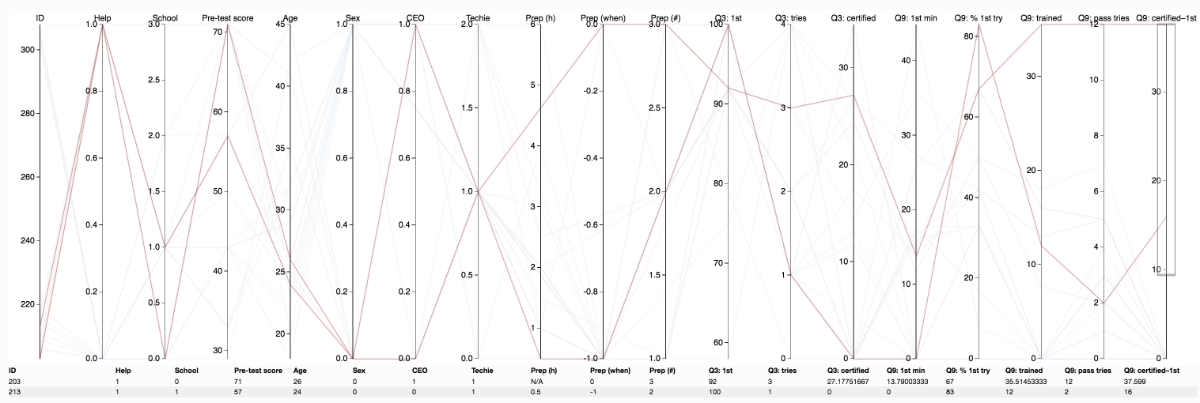
\includegraphics[width=1.0\textwidth]{analysis/paralellCoordinatesWomen.png}
    \caption{The parallel coordinates visualization showing the characteristics of the two coaches that passed the quiz 9 certification. They were both CBTs, they could both could consult the manuals, they had a low education, while still having higher pre-test scores that the average. They were relatively young and were both women (in minority). One had a company and one did not. The one that inserted how she prepared for session, said she prepared the day before (versus doing it the same day), on three occations. Regarding quiz results, they both had a high score on try 1 of quiz 3 "Financial literacy" (1 or 0 errors), just like the majority, and it took them 1 or 3 tries to pass the training. For the coach where time is recorded for getting certified, it took her 27 minutes to pass the quiz (higher than the average). On quiz 9, it took 13 minutes to get 67\%, the other coach (time not known) scoring 83\%. While the coach with 83\% passed the training in only 12 minutes and 2 tries, it was the coach taking 35 minutes to take 12 tries that could afterwards get all of the answers correct in the Certification.}
    \label{fig:quiz9pl}
\end{figure}

Finally, it is interesting to observe the differences (and lack thereof) between the test group and reference group, by following the lines from the second column, "Help", of figure \ref{fig:parallellCoordinates3}. In the test group ("Help" = 1), the paper manuals could be read before improving on the quiz results (not during the actual test) The the reference group ("Help" = 0) were only allowed to observe the right answers within the app, from the score board. In quiz 3, where almost all coaches had 92\% or 100\% immediately, there is no difference observable. However, in quiz 9, the hardest quiz, 5/7 that passed the training were in control group A, and 2/2 that passed the certification were in control group A. An explanation could be that the large amount of questions made the correct answers hard to memorize versus actually learning, or that the ones with manuals felt more supported or motivated because of the extra support. While these findings could be true for a larger sample, further research needs to be done. The same methods of data analysis are increasingly relevant with a larger data set, and there seems to be correlations and tendencies worth looking further into.
